\chapter{Adjoint Simulations}\label{cha:Adjoint-Simulations}

Adjoint simulations are generally performed for two distinct applications.
First, they can be used for earthquake source inversions, especially
earthquakes with large ruptures such as the Sumatra-Andaman event
\citep{LayKanamoriAmmon2005,AmmonJiThio2005,ParkSongTromp2005}. Second,
they can be used to generate finite-frequency sensitivity kernels
that are a critical part of tomographic inversions based upon 3D reference
models \citep{TrTaLi05,LiTr06,TrKoLi08,LiTr08}. In either case, source
parameter or velocity structure updates are sought to minimize a specific
misfit function (e.g., waveform or traveltime differences), and the
adjoint simulation provides a means of computing the gradient of the
misfit function and further reducing it in successive iterations.
Applications and procedures pertaining to source studies and finite-frequency
kernels are discussed in Sections~\ref{sec:Adjoint-simulation-sources}
and \ref{sec:Adjoint-simulation-finite}, respectively. The two related
parameters in the \texttt{Par\_file} are \texttt{SIMULATION\_TYPE}
(1, 2 or 3) and \texttt{SAVE\_FORWARD} (boolean).


\section{Adjoint Simulations for Sources Only (not for the Model)}\label{sec:Adjoint-simulation-sources}

In the case where a specific misfit function is minimized to invert
for the earthquake source parameters, the gradient of the misfit function
with respect to these source parameters can be computed by placing
time-reversed seismograms at the receivers and using them as sources
in an adjoint simulation, and then the value of the gradient is obtained
from the adjoint seismograms recorded at the original earthquake location.

\begin{enumerate}
\item \textbf{Prepare the adjoint sources} \label{enu:Prepare-the-adjoint}

\begin{enumerate}
\item First, run a regular forward simlation (\texttt{SIMULATION\_TYPE =
1} and \texttt{SAVE\_FORWARD = .false.}). You can automatically set
these two variables using the \texttt{\small utils/change\_simulation\_type.pl}
script:
\begin{verbatim}
utils/change_simulation_type.pl -f
\end{verbatim}
and then collect the recorded seismograms at all the stations given
in \texttt{DATA/STATIONS}.

\item Then select the stations for which you want to compute the time-reversed
adjoint sources and run the adjoint simulation, and compile them into
the \texttt{DATA/STATIONS\_ADJOINT} file, which has the same format
as the regular \texttt{DATA/STATIONS} file.

\begin{itemize}
\item Depending on what type of misfit function is used for the source inversion,
adjoint sources need to be computed from the original recorded seismograms
for the selected stations and saved in the \texttt{SEM/} directory
with the format \texttt{NT.STA.?X?.adj}, where \texttt{STA}, \texttt{NT}
are the station name and network code given in the \texttt{DATA/STATIONS\_ADJOINT}
file, and \texttt{?X?}  represents the channel name of a particular
adjoint seismogram where the first letter corresponds to the band code governed by the resolution of simulations, for example, generally \texttt{MX?} for the current resolution of global simulations (see Appendix~\ref{cha:channel-codes} for details). The last letter of channel names is the component name \texttt{E/N/Z}.
\item The adjoint seismograms are in the same format as the original seismogram
(\texttt{NT.STA.?X?.sem?}), with the same start time, time interval
and record length.
\end{itemize}
\item Notice that even if you choose to time reverse only one component
from one specific station, you still need to supply all three components
because the code is expecting them (you can set the other two components
to be zero).
\item Also note that since time-reversal is done in the code itself, no
explicit time-reversing is needed for the preparation of the adjoint
sources, i.e., the adjoint sources are in the same forward time sense
as the original recorded seismograms.
\end{enumerate}

\item \textbf{Set the related parameters and run the adjoint simulation}\\
In the \texttt{DATA/Par\_file}, set the two related parameters to
be \texttt{SIMULATION\_TYPE = 2} and \texttt{SAVE\_FORWARD = .false.}.
More conveniently, use the scripts \texttt{utils/change\_simulation\_type.pl}
to modify the \texttt{Par\_file} automatically (\texttt{change\_simulation\_type.pl
-a}). Then run the solver to launch the adjoint simulation.

\item \textbf{Collect the seismograms at the original source location}\\
After the adjoint simulation has completed successfully, get the seismograms
from directory \texttt{OUTPUT\_FILES}.
%
\begin{itemize}
\item These adjoint seismograms are recorded at the locations of the original
earthquake sources given by the \texttt{DATA/CMTSOLUTION} file, and
have names of the form \texttt{NT.S?????.S??.sem} for the six-component
strain tensor (\texttt{SNN,SEE,SZZ,SNE,SNZ,SEZ}) at these locations,
and \texttt{NT.S?????.?X?.sem} for the three-component displacements
(i.e., \texttt{MXN,MXE,MXZ}) recorded at these locations.
\item \texttt{S?????} denotes the source number; for example, if the original
\texttt{CMTSOLUTION} provides only a point source, then the seismograms
collected will start with \texttt{S00001}.
\item These adjoint seismograms provide critical information for the computation
of the gradient of the misfit function.
\end{itemize}
\end{enumerate}



\section{Adjoint Simulations for Finite-Frequency Kernels (Kernel Simulation)}\label{sec:Adjoint-simulation-finite}

Finite-frequency sensitivity kernels are computed in two successive
simulations (please refer to \citet{LiTr06} and \citet{TrKoLi08} for details).

\begin{enumerate}
\item \textbf{Run a forward simulation with the state variables saved at
the end of the simulation}\\
%
Prepare the \texttt{\small CMTSOLUTION} and \texttt{\small STATIONS}
files, set the parameters \texttt{\small SIMULATION\_TYPE}{\small{}
}\texttt{\small =}{\small{} }\texttt{\small 1} and \texttt{\small SAVE\_FORWARD
=}{\small{} }\texttt{\small .true.} in the \texttt{Par\_file} (\texttt{change\_simulation\_type
-F}), and run the solver.

\begin{itemize}
\item Notice that attenuation is not fully implemented yet for the computation
of finite-frequency kernels; if \texttt{ATTENUATION = .true.} is set
in the \texttt{Par\_file}, only effects on phase shift are accounted for
but not on amplitude of the signals. However, we suggest you use the same
setting for \texttt{ATTENUATION} as for your forward simulations.
\item We also suggest you modify the half duration of the \texttt{CMTSOLUTION}
to be similar to the accuracy of the simulation (see Equation \ref{eq:shortest_period}
or \ref{eq:shortest_period_regional}) to avoid too much high-frequency
noise in the forward wavefield, although theoretically the high-frequency
noise should be eliminated when convolved with an adjoint wavefield
with the proper frequency content.
\item This forward simulation differs from the regular simulations (\texttt{\small SIMULATION\_TYPE}{\small{}
}\texttt{\small =}{\small{} }\texttt{\small 1} and \texttt{\small SAVE\_FORWARD}{\small{}
}\texttt{\small =}{\small{} }\texttt{\small .false.}) described in
the previous chapters in that the state variables for the last time
step of the simulation, including wavefields of the displacement,
velocity, acceleration, etc., are saved to the \texttt{LOCAL\_PATH}
to be used for the subsequent simulation.

\item For regional simulations, the files recording the absorbing boundary
contribution are also written to the \texttt{LOCAL\_PATH} when \texttt{SAVE\_FORWARD
= .true.}.
\end{itemize}


\item \textbf{Prepare the adjoint sources}\\
%
The adjoint sources need to be prepared the same way as described
in Section~\ref{sec:Adjoint-simulation-sources}, item~\ref{enu:Prepare-the-adjoint}.

\begin{itemize}
\item In the case of traveltime finite-frequency kernel for one source-receiver
pair, i.e., point source from the \texttt{CMTSOLUTION}, and one station
in the \texttt{STATIONS\_ADJOINT} list, we supply a sample program
in \texttt{utils/adjoint\_sources/traveltime} to cut a certain portion of the original
displacement seismograms and convert them into the proper adjoint
source to compute the finite-frequency kernel.
\begin{lyxcode}
xcreate\_adjsrc\_traveltime~t1~t2~ifile{[}0-5]~E/N/Z-ascii-files~{[}baz]
\end{lyxcode}
where \texttt{t1} and \texttt{t2} are the start and end time of the
portion you are interested in, \texttt{ifile} denotes the component
of the seismograms to be used (0 for all three components, 1 for east,
2 for north, and 3 for vertical, 4 for transverse, and 5 for radial
component), \texttt{E/N/Z-ascii-files} indicate the three-component
displacement seismograms in the right order, and \texttt{baz} is the
back-azimuth of the station from the event location. Note that \texttt{baz}
is only supplied when \texttt{ifile} = 4 or 5.

\item Similarly, a sample program to compute adjoint sources for amplitude finite-frequency kernels may be found in \texttt{utils/adjoint\_sources/amplitude} and used in the same way as described
for traveltime measurements
\begin{lyxcode}
xcreate\_adjsrc\_amplitude~t1~t2~ifile{[}0-5]~E/N/Z-ascii-files~{[}baz].
\end{lyxcode}
\end{itemize}

For adjoint runs (SIMULATION\_TYPE = 3), the adjoint sources need to be put in the \texttt{SEM/} sub-directory in the root directory of the code.
If your adjoint sources have names of the following form for instance:
\begin{verbatim}
  NET.STA00.MXZ.sem.ascii.adj
  NET.STA00.MXZ.sem.ascii.adj
\end{verbatim}
you will need to rename them to:
\begin{verbatim}
  NET.STA00.MXZ.adj
  NET.STA00.MXZ.adj
\end{verbatim}
i.e., suppress file endings \texttt{.sem.ascii}.
You will also need to create a file called \texttt{STATIONS\_ADJOINT} in the \texttt{DATA/} directory in the root directory of the code. That file can be identical to the \texttt{DATA/STATIONS} file if you had a single station in \texttt{STATIONS}.


\item \textbf{Run the kernel simulation}\\
%
With the successful forward simulation and the adjoint source ready
in \texttt{SEM/}, set \texttt{SIMULATION\_TYPE = 3} and \texttt{SAVE\_FORWARD
= .false.} in the \texttt{Par\_file} (e.g., use: \texttt{utils/change\_simulation\_type.pl -b}),
and rerun the solver.

\begin{itemize}
\item The adjoint simulation is launched together with the back reconstruction
of the original forward wavefield from the state variables saved from
the previous forward simulation, and the finite-frequency kernels
are computed by the interaction of the reconstructed forward wavefield
and the adjoint wavefield.
\item The back-reconstructed seismograms at the original station locations
are saved to the \texttt{OUTPUT\_FILES} directory at the end of the
kernel simulations.
\item These back-constructed seismograms can be compared with the time-reversed
original seismograms to assess the accuracy of the backward reconstruction,
and they should match very well (in the time-reversed sense).
\item The files containing the density, P-wave speed and S-wave speed kernels
are saved in the \texttt{LOCAL\_PATH} with the names of \texttt{proc??????\_reg\_?\_rho(alpha,beta)\_kernel.bin},
where \texttt{proc??????} represents the processor number, and \texttt{reg\_?}
denotes the region these kernels are for, including mantle (\texttt{reg\_1}),
outer core (\texttt{reg\_2}), and inner core (\texttt{reg\_3}). The
output kernels are in the unit of $s/km^{3}$.
\item Note that if you set the flag \texttt{APPROXIMATE\_HESS\_KL = .true.} in
the \texttt{constants.h} file and recompile the solver, the adjoint simulation
also saves files \texttt{proc??????\_reg\_1\_hess\_kernel.bin} which can
be used as preconditioners in the crust-mantle region for iterative inverse
optimization schemes.
\end{itemize}

\item \textbf{Run the boundary kernel simulation}\\
%
If you set the \texttt{SAVE\_BOUNDARY\_MESH = .true.} in
the \texttt{constants.h} file before the simulations, i.e., at the
beginning of step 1, you will get not only the volumetric kernels
as described in step 3, but also boundary kernels for the Earth's
internal discontinuities, such as Moho, 410-km discontinuity, 670-km
discontinuity, CMB and ICB. These kernel files are also saved in the
local scratch directory defined by \texttt{LOCAL\_PATH }and have names
such as \texttt{proc??????\_reg\_1(2)\_Moho(d400,d670,CMB,ICB)\_kernel.bin}.
For a theoretical derivation of the boundary kernels, refer to \citet{TrTaLi05},
and for the visualization of the boundary kernels, refer to Section
\ref{sec:Finite-Frequency-Kernels}.

\item \textbf{Run the anisotropic kernel simulation}\\
%
Instead of the kernels for the isotropic wave speeds, you can also
compute the kernels for the 21 independent components $C_{IJ},\, I,J=1,...,6$
(using Voigt's notation) of the elastic tensor in the (spherical)
geographical coordinate system. This is done by setting \texttt{ANISOTROPIC\_KL}
\texttt{=} \texttt{.true.} in \texttt{constants.h} before step 3.
The definition of the parameters $C_{IJ}$ in terms of the corresponding
components $c_{ijkl},ijkl,i,j,k,l=1,2,3$ of the elastic tensor in
spherical coordinates follows \citet{ChTr07}. The computation of
the anisotropic kernels is only implemented in the crust and mantle
regions. The 21 anisotropic kernels are saved in the \texttt{LOCAL\_PATH}
in one file with the name of \texttt{proc??????\_reg1\_cijkl\_kernel.bin}
(with \texttt{proc??????} the processor number). The output kernels
correspond to perturbation $\delta C_{IJ}$ of the elastic parameters
and their unit is in $s/GPa/km^{3}$. For consistency, the output
density kernels with this option turned on are for a perturbation
$\delta\rho$ (and not $\frac{\delta\rho}{\rho}$) and their unit
is in s / (kg/m$^{3}$) / km$^{3}$. These `primary' anisotropic kernels
can then be combined to obtain the kernels related to other descriptions
of anisotropy. This can be done, for example, when combining the kernel
files from slices into one mesh file (see Section~\ref{sec:Finite-Frequency-Kernels}).

\item \textbf{Run the steady state kernel simulation}\\
%
For source encoded adjoint tomography, you can compute the stationary kernels by enabling the flag \texttt{STEADY\_STATE\_KERNEL}. The kernels will then be computed through the stationary part of the wavefield, as is shown in Figure~\vref{fig:Steady-state-kernel}. The length of the stationary wavefield ($\Delta\tau$ in Figure~\ref{fig:Steady-state-kernel}) can be speified with \texttt{STEADY\_STATE\_LENGTH\_IN\_MINUTES}. Please refer to \citet{bachmann2020source} for details.
%
\begin{figure}[H]
    \begin{centering}
    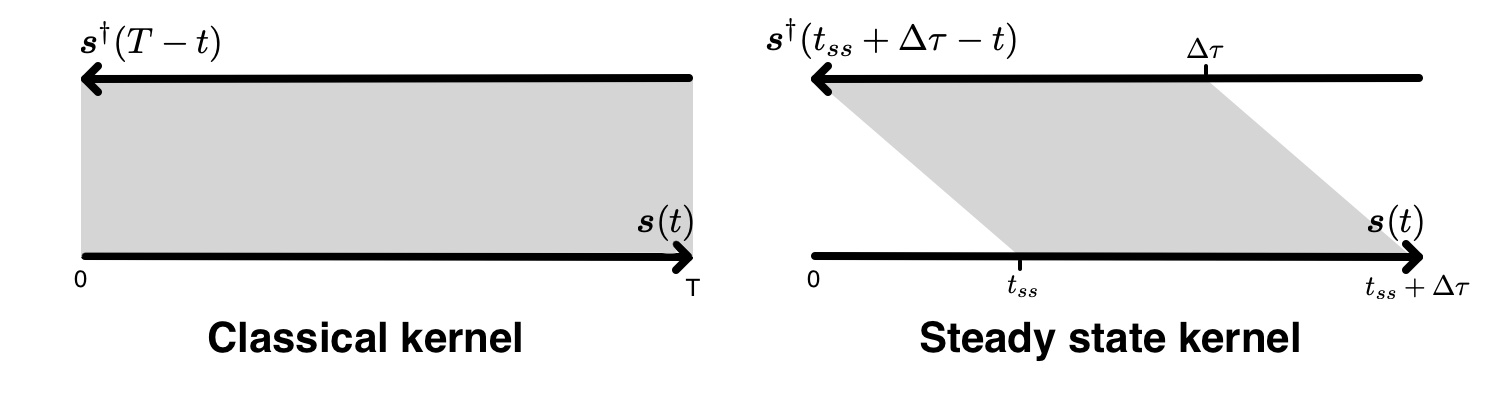
\includegraphics[scale=0.25]{figures/fig7.jpg}
    \par\end{centering}

    \caption{An illustration of computing steady state kernels. Instead of integrating the forward and adjoint wavefields from the beginning, a steady state kernel is computed by integrating the wavefields starting from the time when steady state is reached ($t_{ss}$).}
    \label{fig:Steady-state-kernel}
\end{figure}

\end{enumerate}


In general, the first three steps need to be run sequentially to ensure
proper access to the necessary files at different stages. If the simulations
are run through some cluster scheduling system (e.g., LSF), and the
forward simulation and the subsequent kernel simulations cannot be
assigned to the same set of computer nodes, the kernel simulation
will not be able to access the database files saved by the forward
simulation. Solutions for this problem are provided in Chapter~\ref{cha:Running-Scheduler}.
Visualization of the finite-frequency kernels is discussed in Section~\ref{sec:Finite-Frequency-Kernels}.



